% ----------------------------------------------
%
%	Damian Skrzypiec
% 	20.04.2017
%	Draft of Master Thesis - Mathematics
%
% ----------------------------------------------

\documentclass{pracamgr}


\usepackage[UTF8]{inputenc}
\usepackage{latexsym}
\usepackage{amsmath}
\usepackage{amsthm}
\usepackage{amssymb}

% ----------------------
% For Geogebra
% ----------------------

\usepackage{pgf,tikz}
\usepackage{color}
\usetikzlibrary{arrows}
\usepackage{xcolor}
%\usepackage[latin2]{inputenc}
%\usepackage[utf8]{inputenc}
\usepackage{latexsym}
\usepackage{graphicx,wrapfig,lipsum}
\definecolor{uququq}{rgb}{0.25098039215686274,0.25098039215686274,0.25098039215686274}


% Dane magistranta:

\author{Damian Skrzypiec}

\nralbumu{320335}

\title{Structure Learning Algorithms for Chain Graphs}

\tytulang{}

%kierunek: Matematyka, Informatyka, ...
\kierunek{Mathematics}


% Praca wykonana pod kierunkiem:
% (podać tytuł/stopień imię i nazwisko opiekuna
% Instytut
% ew. Wydział ew. Uczelnia (jeżeli nie MIM UW))
\opiekun{John Noble, PhD.\\
  Institute of Applied Mathematics and Mechanics\\
  }

% miesiąc i~rok:
\date{April 2017}

%Podać dziedzinę wg klasyfikacji Socrates-Erasmus:
\dziedzina{ 
11.2 Statistics\\ 
}

%Klasyfikacja tematyczna wedlug AMS (matematyka) lub ACM (informatyka)
\klasyfikacja{62 Statistics \\
		62C10 Bayesian Problems \\
		}

% Słowa kluczowe:
\keywords{graphical model, chain graph, structure learning}

% Tu jest dobre miejsce na Twoje własne makra i~środowiska:
\newtheorem{defi}{Definition}[section]

% koniec definicji

\begin{document}
\maketitle

\begin{abstract}
  In this place will be abstract of this project.
\end{abstract}

\tableofcontents
%\listoffigures
%\listoftables

\chapter{Introduction}

% ---------------------------------------
%	Damian Skrzypiec
%	IV 2017
%	Introduction
% ---------------------------------------


The purpose of this project is to present algorithms for learning conditional independence structure of joint probability distributions represented by chain graphs. This is a special case of learning probabilistic graphical models which provides convenient representation of factorisation probability distribution using graphs.
Well-known and well-examined examples of probabilistic graphical models (PGMs) are Bayesian Networks where PGM is represented by directed acyclic graph and Markov Fields where PGM is represented by undirected graph. Chain graphs is a class of graphs that does not contains cycles (formal definition in \ref{chainGraphDef}). It contains both directed acyclic graphs and undirected graphs hence it is natural generalization of Bayesian Networks and Markov Fields.
In this paper we present one algorithm for learning chain graphs and one algorithm for learning undirected graphical models. Both algorithms are based on idea of graph decomposition which suppose to decrease complexity of algorithms.


\chapter{Preliminaries}\label{r:prelim}

	\section{Graph Theory Terminology}\label{r:defGraph}s
		% ----------------------------------------------
%
%	Damian Skrzypiec
% 	03.05.2017
%	Graph Theory Definitions
%
% ----------------------------------------------


This section provides definitions of graph theory objects required for completeness of further sections.
In this section, when is not mention different, $V$ is default notation for set of graph's vertices and 
$E$ is default notation for set of graph's edges. 


% ----------------------
% Undirected edge
% ----------------------
\begin{defi} (Undirected edge) \\
	For vertices $u, v \in V$ we say that there is an undirected edge between vertices $u$ 
	and $v$ if $(u, v) \in E$ and $(v, u) \in E$. Undirected edge between $u$ and $v$ is marked as $u-v$.
\end{defi}


% ----------------------
% Directed edge
% ----------------------
\begin{defi} (Directed edge) \\
	For vertices $u, v \in V$ we say that there is a directed edge from vertex $u$ to vertex $v$ if
	$(u, v) \in E$ and $(v, u) \notin E$. Directed edge from $u$ to $v$ is marked as $u \rightarrow v$.
\end{defi}


% ----------------------
% Sekelton
% ----------------------
\begin{defi} (Skeleton) \\
	Skeleton of graph $G = (V, E)$ is a graph $G' = (V', E')$ where $V = V'$ and the set of edges $E'$
	is obtained by replacing directed edges of set $E$ by undirected edges.
\end{defi}


% ----------------------
% Route
% ----------------------
\begin{defi} (Route) \\
	A \textit{route} in graph $G = (V, E)$ is a sequence of vertices $(v_0, \dots, v_k)$, $k \ge 0$, such that 
	$$ (v_{i-1}, v_i) \in E \ \  \mbox{or} \ \ (v_i, v_{i-1}) \in E$$
	for $i = 1, \dots, k$. The vertices $v_0$ and $v_k$ are called \textit{terminals}. A route is called descending
	if $(v_{i-1}, v_i) \in E$ for $i = 1, \dots, k$. Descending route from $u$ to $v$ is marked as $u \mapsto v$. 
\end{defi}


% ----------------------
% Path
% ----------------------
\begin{defi} (Path) \\
	A route $r = (v_0, v_1, \dots, v_k)$ in graph $G = (V, E)$ is called a path if all vertices in $r$ are distinct.
\end{defi}


% ----------------------
% Complex
% ----------------------
\begin{defi} \label{complexDef} (Complex) \\
	A path $\pi = (v_1, v_2, \dots, v_k)$ in graph $G = (V, E)$ is called complex if
	\begin{enumerate}
		\item $v_1 \rightarrow v_2$
		\item $\forall_{i \in \left\{ 2, 3, \dots k-2 \right\}} \ v_i - v_{i+1}$
		\item $v_{k-1} \leftarrow v_k$
		\item There is not additional edges in graph $G$ for vertices in path $\pi$.
	\end{enumerate}
	Vertices $v_1$ and $v_k$ are called \textit{parents} of the complex, set of vertices 
	$\left\{v_2, v_3, \dots, v_{k-1} \right\}$ is called \textit{region} of the complex and number
	$k-2$ is the \textit{degree} of the complex.
\end{defi}
Next we define extended version of moral graphs. In Bayesian Networks moral graph is 
an undirected graph obtained from the original graph by adding undirected edges for not connected parents of the same child and then transform all edges into undirected edges. In case of chain graphs there can be situation when there are 
not connected parents of connected children (see \ref{fig:ImmoralCG}). 
This situation can be interpreted as immoral and to be moralized a connection between parents are required.


\begin{ex} (Immorality in chain graph) \\
	\begin{figure}[h]
		\centering
		\vspace{-10pt}
		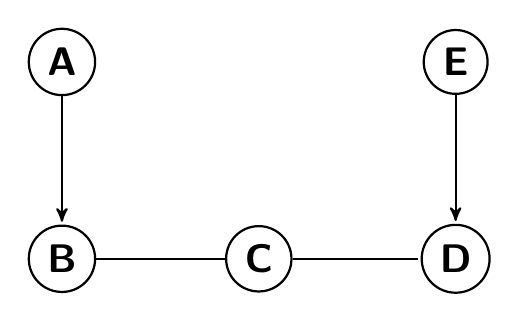
\begin{tikzpicture}[>=stealth',shorten >=1pt,auto,node distance=2.5cm,
		                    thick,main node/.style={circle,draw,font=\sffamily\Large\bfseries}]
			% Nodes
			  \node[main node] (A) {A};
			  \node[main node] (B) [below of = A] {B};
			  \node[main node] (C) [right of = B] {C};
			  \node[main node] (D) [right of = C] {D};
			  \node[main node] (E) [above of = D] {E};
			
			% Edges
			  \draw[->] (A) -- (B);
			  \draw     (B) -- (C) -- (D);
			  \draw[->] (E) -- (D);
			\end{tikzpicture}
			
		\caption{Immorality in chain graph}			
		\label{fig:ImmoralCG} 
	\end{figure}
\end{ex}

% ----------------------
% Moral Graph
% ----------------------
\begin{defi} \label{moralGraphDef} (Moral Graph) \\
	Let $G = (V, E)$ be a graph. A moral graph $G^{m} = (V, E^{m})$ of graph $G$ is a graph obtained by firstly join parents of complexes in graph $G$ and then replace all edges by undirected edges.
\end{defi}


% ----------------------
% Cycles
% ----------------------
\begin{defi} (Cycle) \\
	A route $r = (v_0, v_1, \dots, v_k)$ in graph $G = (V, E)$ is called a pseudocycle if $v_0 = v_k$ and 
	a cycles if further route is a path and $k \ge 3$.
\end{defi}

A graph with only directed edges is called an \textit{undirected graph}. A graph without directed cycles 
and with only directed edges is called a \textit{directed acyclic graph} (DAG).


% ----------------------
% Chain graph
% ----------------------
\begin{defi}\label{chainGraphDef} (Chain graph)  \\
	A graph $G = (V, E)$ is called a chain graph if it does not have directed (pseudo) cycles.
\end{defi}



% ----------------------
% Section
% ----------------------
\begin{defi} (Section) \\
	A subroute $\sigma = (v_i, \dots, v_j)$ of route $\rho = (v_0, \dots, v_k)$ in graph $G$ is called section if $			\sigma$ is the maximal undirected subroute of route $\rho$. That means $v_i - \dots - v_j$ for $0 \le i \le j 			\le k$. Vertices $v_i$ and $v_j$ are called terminals of section $\sigma$. Further vertex $v_i$ is called a 			head-terminal if $i>0$ and $v_{i-1} \rightarrow v_i$ in graph $G$. Analogically vertex $v_j$ is called 
	a head-terminal if $j<k$ and $v_j \leftarrow v_{j+1}$ in graph $G$.
\end{defi}


A section with two head-terminals is called \textit{head-to-head} section. Otherwise the section is called 
\textit{non head-to-head}. For a given set of vertices $S \subset V$ in graph $G$ and section $\sigma = (v_i, \dots, v_j)$ we say that section is hit by $S$ if $\left\lbrace v_i , \dots, v_j \right\rbrace \cap S \neq \emptyset$. Otherwise we say that section $\sigma$ is outside set $S$.



% ----------------------
% Intervention
% ----------------------
\begin{defi} (Intervention) \\
	A route $\rho$ in graph $G = (V, E)$ is blocked by a subset $S \subset V$ of vertices if and only if there 				exists a section $\sigma$ of route $\rho$ such that one of the following conditions is satisfied.
	
	\begin{enumerate}
		\item Section $\sigma$ is head-to-head with respect to $\rho$ and $\sigma$ is outside of $S$.
		\item Section $\sigma$ is non head-to-head with respect to $\rho$ and $\sigma$ is hit by $S$.
	\end{enumerate}
	
\end{defi}



\begin{ex} (Graph definitions) \\
	Based on the following two graphs (figures \ref{fig:ExampleGraph} and \ref{fig:ExampleMoralGraph}) we 
	present examples of above defined definitions. Let graph 
	presented in figure \ref{fig:ExampleGraph} be denoted as $G$. In graph $G$ as example of descending 
	route is $(A, B, C, D)$ and 
	example of non-descending route is $(D, E, F, G)$. Graph $G$ contains two complexes. Complex $(A, B, C, D, E)$
	is of degree equal to $3$ and the other one $(F, G, H, I)$ is of degree equal to $2$. Graph $G$ contains one cycle
	$(I, J, K, I)$. The Route $(F, G, H, I)$ in graph $G$ contains section $(G, H)$ which is head-to-head section.

	\begin{figure}[h]
		\centering
		\vspace{-10pt}
		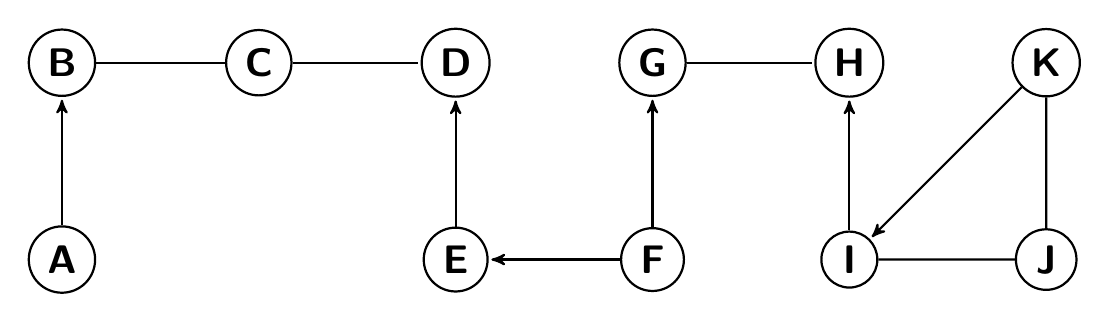
\begin{tikzpicture}[>=stealth',shorten >=1pt,auto,node distance=2.5cm,
		                    thick,main node/.style={circle,draw,font=\sffamily\Large\bfseries}]
			% Nodes
			  \node[main node] (A) {A};
			  \node[main node] (B) [above of = A] {B};
			  \node[main node] (C) [right of = B] {C};
			  \node[main node] (D) [right of = C] {D};
			  \node[main node] (E) [below of = D] {E};
			  \node[main node] (F) [right of = E] {F};
			  \node[main node] (G) [above of = F] {G};
			  \node[main node] (H) [right of = G] {H};
			  \node[main node] (I) [below of = H] {I};
			  \node[main node] (J) [right of = I] {J};
			  \node[main node] (K) [above of = J] {K};
			
			% Edges
			  \draw[->] (A) -- (B);
			  \draw     (B) -- (C) -- (D);
			  \draw[->] (E) -- (D);
			  \draw[->] (F) -- (E);
			  \draw[->] (F) -- (G);
			  \draw     (G) -- (H);
			  \draw[->] (I) -- (H);
			  \draw[->] (I) -- (J) -- (K) -- (I);
			\end{tikzpicture}
			
		\caption{Example graph}			
		\label{fig:ExampleGraph} 
	\end{figure}
	
	Graph presented in figure \ref{fig:ExampleMoralGraph} is moral graph of graph $G$. 
	Additional undirected edges $A - E$ and $F - I$ are the result of connecting parents of complexes in 
	the original graph $G$.
	
	\begin{figure}
	 	\centering
	 	\vspace{-10pt}
	 	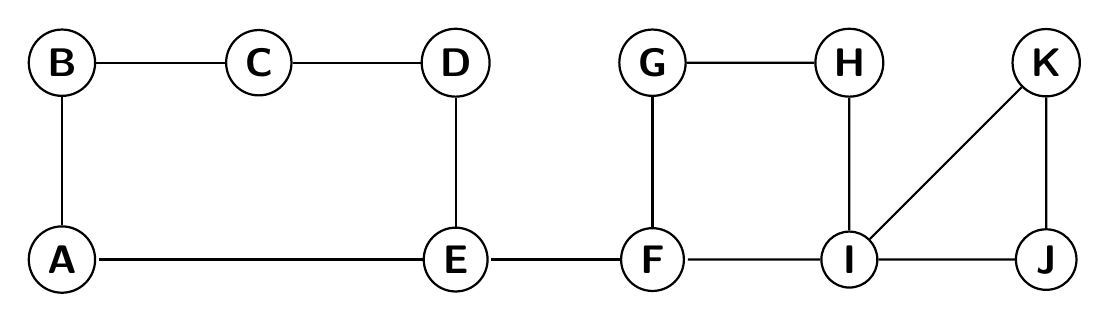
\begin{tikzpicture}[>=stealth',shorten >=1pt,auto,node distance=2.5cm,
		                    thick,main node/.style={circle,draw,font=\sffamily\Large\bfseries}]
			% Nodes
			  \node[main node] (A) {A};
			  \node[main node] (B) [above of = A] {B};
			  \node[main node] (C) [right of = B] {C};
			  \node[main node] (D) [right of = C] {D};
			  \node[main node] (E) [below of = D] {E};
			  \node[main node] (F) [right of = E] {F};
			  \node[main node] (G) [above of = F] {G};
			  \node[main node] (H) [right of = G] {H};
			  \node[main node] (I) [below of = H] {I};
			  \node[main node] (J) [right of = I] {J};
			  \node[main node] (K) [above of = J] {K};
			
			% Edges
			 \draw (A) -- (B) -- (C) -- (D) -- (E) -- (A);
			 \draw (G) -- (F) -- (E);
			 \draw (F) -- (G) -- (H) -- (I) -- (J) -- (K) -- (I) -- (F);
			\end{tikzpicture}
			
		\caption{Moral graph of graph in figure \ref{fig:ExampleGraph}}			
		\label{fig:ExampleMoralGraph} 
    \end{figure}		
	
	
\end{ex}




		
	\section{Graphical Model Terminology}\label{r:defGraphModel}
		
% ----------------------
% Conditional independence
% ----------------------
%
Our main goal is to find an conditional independence structure of given joint probability distribution, hence we start from recalling definition of conditional independence.

\begin{defi} \label{condInd} (Conditional Independence) \\
	Let $(X_1, X_2, \dots, X_n)$ be a random vector over probability space $(\Omega, \mathcal{F}, \mathbb{P})$.
	We say that random vectors $X_A = \left\{ X_a  \ | \ a \in A \right\}$ and 
	$X_B = \left\{ X_b  \ | \ b \in B \right\}$
	are conditional independent given $X_S = \left\{ X_s  \ | \ s \in S \right\}$ when 
	for all $A_1, A_2, A_3 \in \mathcal{F}$
	%
	\begin{equation} 
		\mathbb{P}(X_A \in A_1, X_B \in A_2 \mid X_S \in A_3) = \mathbb{P}(X_A \in A_1 \mid X_S \in A_3) 													\mathbb{P}(X_B \in A_2 \mid X_S \in A_3)
	\end{equation}
	%
	where $A, B, S \subset {1, 2, \dots, n}$. Conditional independence of $X_A$ and $X_B$
	given $X_S$ is denoted as $X_A \bigCI X_B \mid X_S$.
\end{defi}
The following definition of c-separation is an analogical version of d-separation, used in Bayesian Networks, for chain graphs. This definition was introduced by Studeny and Bouckaert in \cite{OCG}. The notation c-separation is short of "chain separation" and it is written in this form to present analogy to definition of d-separation.


% ----------------------
% c-separation
% ----------------------
\begin{defi} \label{cSepDef} (c-separation) \\
	Let $G = (V, E)$ be a chain graph. Let $A, B, S$ be three disjoint subsets of the vertex set $V$, such that
	$A$ and $B$ are nonempty. We say that $A$ and $B$ are c-separated by $S$ on $G$ if every route within one of 
	its terminals in $A$ and the other in $B$ is blocked by $S$. 
	We call $S$ a c-separator for $A$ and $B$ and mark as \cSep{A}{B}{S}{G}.
\end{defi}


% ----------------------
% Faithfulness and Markovian
% ----------------------
\begin{defi} \label{faithDef} (faithfulness) \\
	Let $G = (V, E)$ be a chain graph with random variables $X_v$ associated with vertex $v \in V$. Let note domain of 
	random variable $X_v$ as $\mathcal{X}_v$. A probability measure $\mathbb{P}$ 
	defined on $\prod_{v \in V} \mathcal{X}_v$ is \textit{faithful} with respect to $G$ if 
	for any triple $(A, B, S)$ of disjoint subsets of $V$ where $A$ and $B$ are non-empty we have
	%
	\begin{equation}
		\cSep{A}{B}{S}{G} \iff X_A \bigCI X_B \mid X_S
	\end{equation}
	%	
	In the same setup a probability measure $\mathbb{P}$ is called \textit{Markovian} with respect to $G$ if
	%
	\begin{equation}
		\cSep{A}{B}{S}{G} \Longrightarrow X_A \bigCI X_B \mid X_S
	\end{equation}
	%
\end{defi}

\begin{remark}
	\normalfont
	In the further section of this paper we will use c-separation statement for some chain graph $G$ even if
	at that time graph $G$ is unknown. In such a situation it should be interpreted as c-separation statement under 
	probability distribution $\mb{P}$ which is faithful to graph $G$. In particular in the chapter 3
	we will be using separation trees, which depends on chain graph $G$, to build chain graph $G$ via LCD algorithm.
	Underlying meaning is that separation trees are built based on probability distribution that is faithful to 
	chain graph $G$ but we do not know form of graph $G$ beforehand. 
\end{remark}


The following theorem from Frydenberg's paper \cite{CGMP} provides convenient tool for testing if two given 
chain graphs are the same in respect to Markov equivalent class.

% ----------------------
% Markov equivalence of chain graphs
% ----------------------
\begin{prop} \label{markovEquivThm} (Markov equivalence of chain graphs) [Theorem 5.6 from \cite{CGMP}] \\
	Two chain graphs $G_1 = (V_1, E_1)$ and $G_2 = (V_2, E_2)$ have the same Markov properties if and only if they same 
	the same skeleton and the same complexes.
\end{prop}	






\chapter{Structural Learning of Chain Graphs}

	\section{Algorithm}


\chapter{Undirected Graphical Model Selection}
	
	\section{Algorithm}


\begin{thebibliography}{99}
	\addcontentsline{toc}{chapter}{Bibliography}
	\bibitem{UGM} R. D. Nowak and D. Vats, \textit{A Junction Tree Framework for Undirected Graphical Model Selection}, Journal of Machine Learning Research 15 (2014) 147-191
	
	\bibitem{CG} Z. Ma, X. Xie and Z. Geng, \textit{Structural Learning Of Chain Graphs via Decomposition}, Journal of Machine Learning Research 9 (2008) 2847-2880
	
\end{thebibliography}

\end{document}


%%% Local Variables:
%%% mode: latex
%%% TeX-master: t
%%% coding: latin-2
%%% End:
